%!TEX TS-program = xelatex
%!TEX encoding = UTF-8 Unicode
\documentclass[12pt,a4paper]{article}
\usepackage{geometry} % 設定邊界
\geometry{
  top=1in,
  inner=1in,
  outer=1in,
  bottom=1in,
  headheight=3ex,
  headsep=2ex
}
\usepackage{fontspec} % 允許設定字體
\usepackage{xeCJK} % 分開設置中英文字型
\usepackage{url} % 使用url
\setCJKmainfont{LiHei Pro} % 設定中文字型
\setmainfont{Georgia} % 設定英文字型
\setromanfont{Georgia} % 字型
\setmonofont{Courier New}
\linespread{1.2}\selectfont % 行距
\XeTeXlinebreaklocale "zh" % 針對中文自動換行
\XeTeXlinebreakskip = 0pt plus 1pt % 字與字之間加入0pt至1pt的間距,確保左右對整齊
\parindent 0em % 段落縮進
\setlength{\parskip}{20pt} % 段落之間的距離

\title{\huge 影像處理 Assignment3 - 去除影像雜訊} % 設置標題,使用巨大字體
\author{姓名:吳嘉偉\quad 學號:5105056013\quad 日期:2017/12/31} % 設置作者
\date{} % 設置日期
\usepackage{titling}
\setlength{\droptitle}{-8em} % 將標題移動至頁面的上面
\usepackage{listings}

\begin{document}

\clearpage

\maketitle % 顯示標題

\section{產生雜訊}

\subsection{胡椒鹽雜訊 Pepper salt noise}

{
\fontsize{14pt}{10pt} % 字型大小14pt,字行間距20pt
\selectfont % 生效
隨機產生白色或黑色的雜訊,像是灑胡椒鹽在影像上,
此作業是使用1/2的機率產生雜訊
\begin{figure}[ht]
\centering
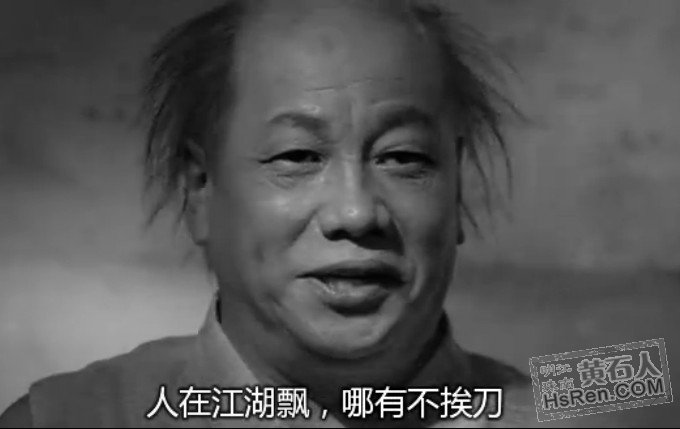
\includegraphics[width=.5\textwidth]{image/gray_image.png}
\hspace{1cm}
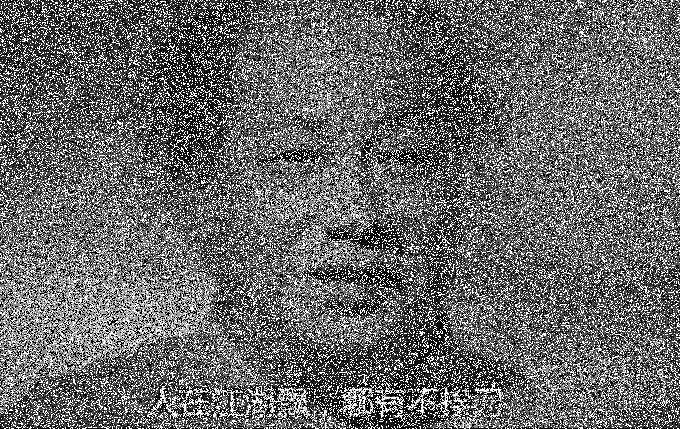
\includegraphics[width=.5\textwidth]{image/noise_Image.png}
\caption{Source and Noise Image}%整個標籤
\label{要合併的兩張圖}%整個圖形標籤
\end{figure}
}

\newpage % 新一頁
\subsection{程式碼}

{
\begin{lstlisting}[language=Python]

# 加上雜訊
def addNoiseWithPercent(image, percent=0):
    if percent == 0:
        savePhoto('noise_Image', image)
        return image

    height = image.shape[0]
    width = image.shape[1]
    newImage = np.zeros((height, width, 3), np.uint8)
    for x in range(width):
        for y in range(height):
            ran = random.randint(1, 10)
            if ran % 10 < percent:
                noiseRan = random.randint(1, 10)
                if noiseRan % 2 == 0:
                    newImage[y][x] = 0
                else:
                    newImage[y][x] = 255
            else:
                newImage[y][x] = image[y][x]

    savePhoto('noise_Image', newImage)
    return newImage
\end{lstlisting}
}

\newpage % 新一頁
\section{Median Filter Algorithm}
\subsection{取得參數}
{
先取得Zmin, Zmax, Zmed, Zxy的數值

程式碼
\begin{lstlisting}[language=Python]

# 取得zMax, zMed, zMin, zXY各個值
def getGrayLevelValue(image, x, y, mask=3):
    height = image.shape[0]
    width = image.shape[1]
    pixels = []

    for j in range(mask):
        pixelY = y - mask // 2 + j
        if pixelY < 0 or pixelY >= height:
            continue
        for i in range(mask):
            pixelX = x - mask // 2 + i
            if pixelX < 0 or pixelX >= width:
                continue
            pixels.append(image[pixelY][pixelX][0])

    pixels.sort()
    zMin = pixels[0]
    zMax = pixels[-1]
    med = len(pixels) // 2
    zMed = pixels[med]
    zXY = image[y][x][0]
    return zMax, zMed, zMin, zXY
\end{lstlisting}
}

\newpage
\subsection{實現Median Filter}
{
依照講義上的Pseudo Code

程式碼
\begin{lstlisting}[language=Python]

# 做Median Filter
def adaptiveMedianFilter(image, x, y, size=3, sizeMax=7):
    zMax, zMed, zMin, zXY = getGrayLevelValue(image, x, y, size)
    # LevelA
    a1 = int(zMed) - int(zMin)
    a2 = int(zMed) - int(zMax)
    if a1 > 0 and a2 < 0:
    # if zMin < zMed < zMax:
        # Level B
        b1 = int(zXY) - int(zMin)
        b2 = int(zXY) - int(zMax)
        if b1 > 0 and b2 < 0:
        # if zMin < zXY < zMax:
            return zXY
        else:
            return zMed
    else:
        newSize = size + 2

    if newSize <= sizeMax:
        # repeat LevelA
        return adaptiveMedianFilter(image, x, y, newSize)
    else:
        return zXY
\end{lstlisting}
}

\newpage
\section{結論}
去掉雜訊後與原圖比較,還是會有些許的雜訊無法去除。
而且文字是比較難以還原的。
\begin{figure}[ht]
\centering
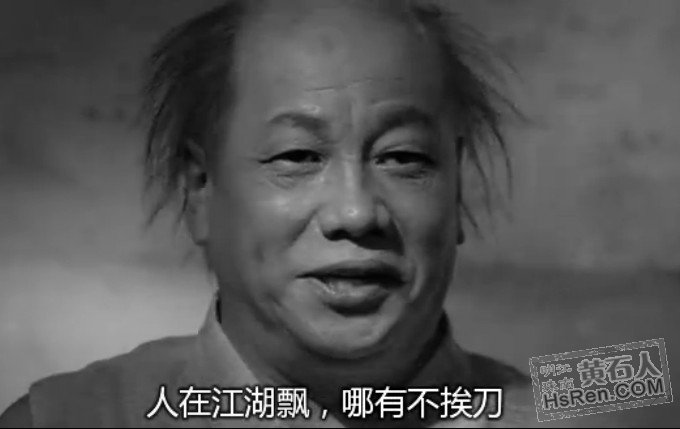
\includegraphics[width=.8\textwidth]{image/gray_image.png}
\caption{Source Image}%整個標籤
\label{合併影像}%整個圖形標籤
\end{figure}
\begin{figure}[ht]
\centering
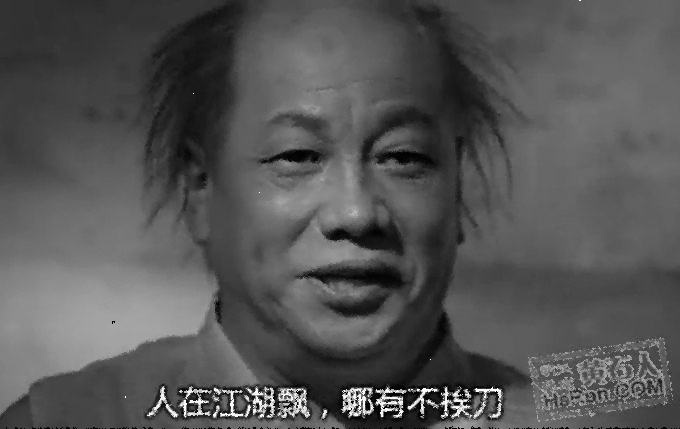
\includegraphics[width=.8\textwidth]{image/filterNoise_Image.png}
\caption{Filter Image}%整個標籤
\label{合併影像}%整個圖形標籤
\end{figure}
\end{document}